\documentclass[border=0.125cm]{standalone}
\usepackage{tikz}
\usepackage{pgfplots}
\usepackage{graphicx}

\usetikzlibrary{decorations.pathmorphing}
\pgfplotsset{compat=newest}
\usetikzlibrary{shapes.geometric,arrows,fit,matrix,positioning}
\tikzset{main node/.style={circle,fill=black!20,draw,minimum size=3.5mm,inner sep=0pt},
         every node/.style={circle,fill=black,draw,minimum size=1mm,inner sep=0pt,label distance=-1mm},
         subtree/.style={isosceles triangle,fill=black!20,draw,minimum size=5mm,inner sep=0pt,shape border rotate=90},
         edge label/.style = {rectangle,draw=none,fill=none},
         blank edge/.style={edge from parent/.style={draw=none}},
         norm edge/.style={edge from parent/.style={black,thin,draw}},
}
\begin{document}
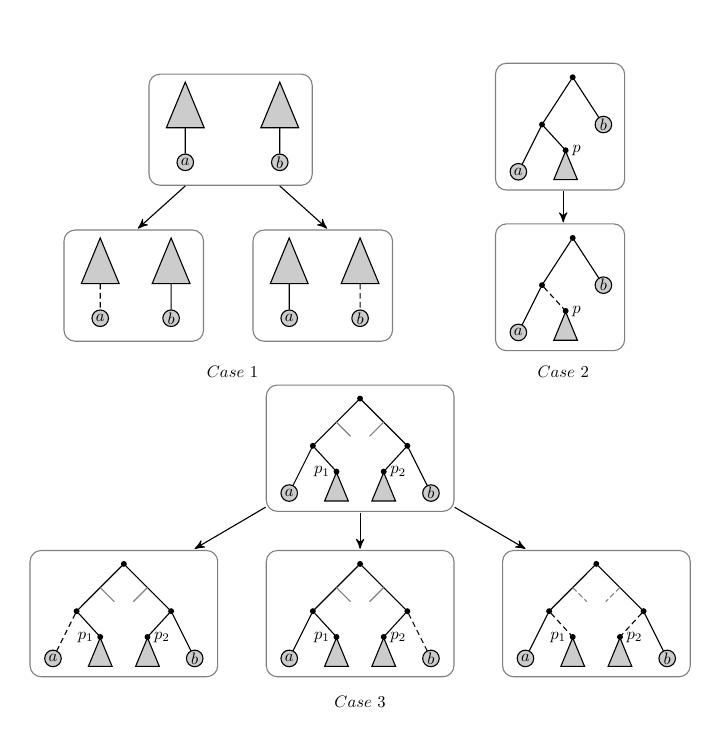
\begin{tikzpicture}[-,>=stealth', 
level 1/.style={sibling distance = 20mm},
level distance = 1cm, 
scale=0.6,
transform shape]

% \draw[help lines] (-2,0) grid (15,-15);

\node[subtree,minimum size = 8mm] (t1_0) at (2.8,-1) {}
    child[edge from parent path = {(\tikzparentnode.south) -- (\tikzchildnode)}]{
        node[main node] (t1_1) {$a$}
    }
;

\node[subtree,minimum size = 8mm] (t2_0) at (4.8,-1) {}
    child[edge from parent path = {(\tikzparentnode.south) -- (\tikzchildnode)}]{
        node[main node] (t2_1) {$b$}
    }
;

\node[subtree,minimum size = 8mm] (1t1_0) at (1,-4.3) {}
    child[edge from parent path = {(\tikzparentnode.south) -- (\tikzchildnode)[dash pattern=on 2pt off 1.3pt]}]{
        node[main node] (1t1_1) {$a$}
    }
;

\node[subtree,minimum size = 8mm] (1t2_0) at (2.5,-4.3) {}
    child[edge from parent path = {(\tikzparentnode.south) -- (\tikzchildnode)}]{
        node[main node] (1t2_1) {$b$}
    }
;

\node[subtree,minimum size = 8mm] (2t1_0) at (5,-4.3) {}
    child[edge from parent path = {(\tikzparentnode.south) -- (\tikzchildnode)}]{
        node[main node] (2t1_1) {$a$}
    }
;

\node[subtree,minimum size = 8mm] (2t2_0) at (6.5,-4.3) {}
    child[edge from parent path = {(\tikzparentnode.south) -- (\tikzchildnode)[dash pattern=on 2pt off 1.3pt]}]{
        node[main node] (2t2_1) {$b$}
    }
;

\node[edge label,above left = 6mm and 5mm of t1_0] (pos_1) {};   
\node[edge label,below right = 3mm and 5mm of t2_1] (pos_2){};
\draw[rounded corners,gray] (pos_1) rectangle (pos_2);

\node[edge label,above left = 6mm and 5mm of 1t1_0] (1pos_1) {};   
\node[edge label,below right = 3mm and 5mm of 1t2_1] (1pos_2){};
\draw[rounded corners,gray] (1pos_1) rectangle (1pos_2);

\node[edge label,above left = 6mm and 5mm of 2t1_0] (2pos_1) {};   
\node[edge label,below right = 3mm and 5mm of 2t2_1] (2pos_2){};
\draw[rounded corners,gray] (2pos_1) rectangle (2pos_2);

\draw[->] (2.8,-2.5) -- (1.8,-3.4);
\draw[->] (4.8,-2.5) -- (5.8,-3.4);

\node [edge label, xshift = 0mm, below=63mm, align=flush center] at (3.8,0){
        {$Case~1$}};


\node[edge label] at (11,0.8) {}
child[blank edge]{
    [sibling distance = 13mm]node (c2_t_0) {}
        child[norm edge]{
            [sibling distance = 10mm] node (c2_t_1) {}
                child{
                    node [main node] (c2_t_2) {$a$}
                }
                child[edge from parent path = {(\tikzparentnode) -- (\tikzchildnode.north)}]{
                    node [subtree] (c2_t_3) {}
                }
        }
        child[norm edge]{
            node [main node] (c2_t_4) {$b$}
        }
}
;
\node[edge label,above right = 2mm and 0 mm of c2_t_3] {$p$};
\node at (c2_t_3.north) {};
\node[edge label,below left = 2mm and 3mm of c2_t_2] (c2pos_1) {};   
\node[edge label,above right = 2mm and 10mm of c2_t_0] (c2pos_2){};
\draw[rounded corners,gray] (c2pos_1) rectangle (c2pos_2);

\node[edge label] at (11,-2.6) {}
child[blank edge]{
    [sibling distance = 13mm]node (1c2_t_0) {}
        child[norm edge]{
            [sibling distance = 10mm] node (1c2_t_1) {}
                child{
                    node [main node] (1c2_t_2) {$a$}
                }
                child[edge from parent path = {(\tikzparentnode) -- (\tikzchildnode.north)[dash pattern=on 2pt off 1.3pt]}]{
                    node [subtree] (1c2_t_3) {}
                }
        }
        child[norm edge]{
            node [main node] (1c2_t_4) {$b$}
        }
}
;
\node[edge label,above right = 2mm and 0 mm of 1c2_t_3] {$p$};
\node at (1c2_t_3.north) {};
\node[edge label,below left = 2mm and 3mm of 1c2_t_2] (1c2pos_1) {};   
\node[edge label,above right = 2mm and 10mm of 1c2_t_0] (1c2pos_2){};
\draw[rounded corners,gray] (1c2pos_1) rectangle (1c2pos_2);
\draw[->] (10.8,-2.6) -- (10.8,-3.27);
\node [edge label, xshift = 0mm, below=63mm, align=flush center] at (10.8,0){
        {$Case~2$}};


\node (c3_t_0) at (6.5,-7) {}
    child{
        [sibling distance = 10mm] node (c3_t_1) {}
            child{
                node [main node] (c3_t_2) {$a$}
            }
            child[edge from parent path = {(\tikzparentnode) -- (\tikzchildnode.north)}]{
                node [subtree] (c3_t_3) {}
            }
    }
    child{
        [sibling distance = 10mm] node (c3_t_4) {}
            child[edge from parent path = {(\tikzparentnode) -- (\tikzchildnode.north)}]{
                node [subtree] (c3_t_5) {}
            }
            child{
                node [main node] (c3_t_6) {$b$}
            }
    }
;
\node at (c3_t_3.north) {};
\node at (c3_t_5.north) {};
\node[edge label,above left = 2mm and 0 mm of c3_t_3] {$p_1$};
\node[edge label,above right = 2mm and 0 mm of c3_t_5] {$p_2$};
\draw[gray] (6,-7.5) -- (6.3,-7.8);
\draw[gray] (7,-7.5) -- (6.7,-7.8);


\node (c3_t1_0) at (1.5,-10.5) {}
    child{
        [sibling distance = 10mm] node (c3_t1_1) {}
            child[edge from parent path = {(\tikzparentnode) -- (\tikzchildnode)[dash pattern=on 2pt off 1.3pt]}]{
                node [main node] (c3_t1_2) {$a$}
            }
            child[edge from parent path = {(\tikzparentnode) -- (\tikzchildnode.north)}]{
                node [subtree] (c3_t1_3) {}
            }
    }
    child{
        [sibling distance = 10mm] node (c3_t1_4) {}
            child[edge from parent path = {(\tikzparentnode) -- (\tikzchildnode.north)}]{
                node [subtree] (c3_t1_5) {}
            }
            child{
                node [main node] (c3_t1_6) {$b$}
            }
    }
;
\node at (c3_t1_3.north) {};
\node at (c3_t1_5.north) {};
\node[edge label,above left = 2mm and 0 mm of c3_t1_3] {$p_1$};
\node[edge label,above right = 2mm and 0 mm of c3_t1_5] {$p_2$};
\draw[gray] (1,-11) -- (1.3,-11.3);
\draw[gray] (2,-11) -- (1.7,-11.3);

\node (c3_t2_0) at (6.5,-10.5) {}
    child{
        [sibling distance = 10mm] node (c3_t2_1) {}
            child{
                node [main node] (c3_t2_2) {$a$}
            }
            child[edge from parent path = {(\tikzparentnode) -- (\tikzchildnode.north)}]{
                node [subtree] (c3_t2_3) {}
            }
    }
    child{
        [sibling distance = 10mm] node (c3_t2_4) {}
            child[edge from parent path = {(\tikzparentnode) -- (\tikzchildnode.north)}]{
                node [subtree] (c3_t2_5) {}
            }
            child[edge from parent path = {(\tikzparentnode) -- (\tikzchildnode)[dash pattern=on 2pt off 1.3pt]}]{
                node [main node] (c3_t2_6) {$b$}
            }
    }
;
\node at (c3_t2_3.north) {};
\node at (c3_t2_5.north) {};
\node[edge label,above left = 2mm and 0 mm of c3_t2_3] {$p_1$};
\node[edge label,above right = 2mm and 0 mm of c3_t2_5] {$p_2$};
\draw[gray] (6,-11) -- (6.3,-11.3);
\draw[gray] (7,-11) -- (6.7,-11.3);

\node (c3_t3_0) at (11.5,-10.5) {}
    child{
        [sibling distance = 10mm] node (c3_t3_1) {}
            child{
                node [main node] (c3_t3_2) {$a$}
            }
            child[edge from parent path = {(\tikzparentnode) -- (\tikzchildnode.north)[dash pattern=on 2pt off 1.3pt]}]{
                node [subtree] (c3_t3_3) {}
            }
    }
    child{
        [sibling distance = 10mm] node (c3_t3_4) {}
            child[edge from parent path = {(\tikzparentnode) -- (\tikzchildnode.north)[dash pattern=on 2pt off 1.3pt]}]{
                node [subtree] (c3_t3_5) {}
            }
            child{
                node [main node] (c3_t3_6) {$b$}
            }
    }
;
\node at (c3_t3_3.north) {};
\node at (c3_t3_5.north) {};
\node[edge label,above left = 2mm and 0 mm of c3_t3_3] {$p_1$};
\node[edge label,above right = 2mm and 0 mm of c3_t3_5] {$p_2$};
\draw[dash pattern=on 2pt off 1pt,gray] (11,-11) -- (11.3,-11.3);
\draw[dash pattern=on 2pt off 1pt,gray] (12,-11) -- (11.7,-11.3);

\node[edge label,below left = 2mm and 3mm of c3_t_2] (c3pos_1) {};   
\node[edge label,above right = 21mm and 3mm of c3_t_6] (c3pos_2){};
\draw[rounded corners,gray] (c3pos_1) rectangle (c3pos_2);

\node[edge label,below left = 2mm and 3mm of c3_t1_2] (1c3pos_1) {};   
\node[edge label,above right = 21mm and 3mm of c3_t1_6] (1c3pos_2){};
\draw[rounded corners,gray] (1c3pos_1) rectangle (1c3pos_2);

\node[edge label,below left = 2mm and 3mm of c3_t2_2] (2c3pos_1) {};   
\node[edge label,above right = 21mm and 3mm of c3_t2_6] (2c3pos_2){};
\draw[rounded corners,gray] (2c3pos_1) rectangle (2c3pos_2);

\node[edge label,below left = 2mm and 3mm of c3_t3_2] (3c3pos_1) {};   
\node[edge label,above right = 21mm and 3mm of c3_t3_6] (3c3pos_2){};
\draw[rounded corners,gray] (3c3pos_1) rectangle (3c3pos_2);

\draw[->] (4.5,-9.3) -- (3,-10.18);
\draw[->] (8.5,-9.3) -- (10,-10.18);
\draw[->] (6.5,-9.42) -- (6.5,-10.18);

\node [edge label, xshift = 0mm, below=63mm, align=flush center] at (c3_t_0){
        {$Case~3$}};

\end{tikzpicture}

\end{document}



















